\documentclass{article}

% Appearance
%--------------------------------------
\usepackage[a4paper,width=170mm,top=18mm,bottom=22mm,includeheadfoot,marginparsep=2cm]{geometry}
\usepackage{url}
%--------------------------------------

% Colors
%--------------------------------------
\usepackage{color}
\definecolor{lightyellow}{rgb}{1,0.98,0.9}
%--------------------------------------

% Language
%--------------------------------------
\usepackage[utf8]{inputenc}
\usepackage[T2A]{fontenc}
\usepackage{hyphenat}
\hyphenation{he-lio-trope opos-sum}
%--------------------------------------

% References
%--------------------------------------
\usepackage{biblatex}
\addbibresource{biblio.bib}
%--------------------------------------

% Footnotes
%--------------------------------------
\usepackage[hang]{footmisc}
\setlength{\footnotemargin}{14pt}
\setlength{\skip\footins}{20pt}
%--------------------------------------

% Columns
%--------------------------------------
\usepackage{multicol}
\setlength{\columnsep}{24pt}
%--------------------------------------

% Graphics
%--------------------------------------
\usepackage{graphicx}
\graphicspath{{images/}}
%--------------------------------------

% Tables
%--------------------------------------
\usepackage{array, tabularx, caption, boldline}
\usepackage{graphicx}
\usepackage{cellspace}
\usepackage{makecell}
\renewcommand\theadfont{\normalfont\bfseries}
\def\arraystretch{1.5}
%--------------------------------------

% Math
%--------------------------------------
\usepackage{amsmath}
%--------------------------------------

\title{BankEx Proof-of-Asset Protocol}
\author{Yellow Paper, version 0.1.1 alpha}
\date{August 30, 2017}

\begin{document}

%\pagecolor{lightyellow}

\maketitle

\begin{abstract}
BankEx Proof-of-Asset protocol of assets tokenization and liquidity increase are being described. Practical implementation of the Proof-of-Asset Protocol based on Ethereum platform smart-contracts are being described enlightening technical and economical aspects of protocol.
\end{abstract}

\vspace{24pt}

\begin{multicols}{2}

\section{Introduction}

\subsection{BankEx Proof-of-Asset Protocol}

BankEx is an organization uniting members of the financial market in order to build a community and implement the Proof-of-Asset Protocol for the community members to receive profit from mutual use of assets. 

The product of BankEx is the Proof-of-Asset Protocol, which solves the issue of asset liquidity. Proof-of-Asset means the token released as part of the protocol is ensured with an asset. 
The know-how of BankEx is the Proof-of-Asset protocol, in essence a combination of BaaS (Bank-as-a-Service) and blockchain technologies. We take a client asset, primarily on the financial market, we tokenize it, then, without waiting for the portfolio to accumulate critical mass, we turn this asset into money for the bank.  This is made possible because we form a single pool of similar assets, for instance, in a hundred banks and end up with a marketplace, where on the one side we have banks in need of liquidity, and on the other – investors, needing a predictable and transparent cash flow.

\subsection{Specification of examples in Yellow Paper}

Please bear in mind that in this BankEx White Paper all examples and demonstrations featured in the text are used only as demonstrative examples of the SmartDeal technology. The business of BankEx involves manufacturing fintech products and tokenizing primarily financial assets, although we do not think it impossible to apply the Proof-of-Asset Protocol in other fields, with approval from the BankEx Foundation in case of non-financial Smart Assets. In our case, first and foremost we create liquidity for financial assets.

\subsection{Game theory behind the Proof-of-Asset protocol}

Game Theory\footnote{Game theory is the study of the ways in which interacting choices of economic agents produce outcomes with respect to the preferences (or utilities) of those agents, where the outcomes in question might have been intended by none of the agents.\\\url{https://plato.stanford.edu/entries/game-theory/}} is a branch of mathematical economics focusing on the outcomes of conflicts between players, and the optimality of their strategies. Analysis carried out according to game theory indicates that the global financial market is currently trapped in the sub-optimal equilibrium of the prisoner’s dilemma. This dilemma is a fundamental problem of game theory, illustrating how players will sometimes fail to cooperate even if it was in their best interest.

We see that players in financial markets distrust each other and keep overpaying for an inefficient set of various ratings, scores and audits, although these are frequently wrong (as with the Enron scandal and the subprime mortgage crisis). This inefficiency leads to high costs and often losses, which in turn raise the cost of capital and lead to a lack of access to capital for decentralized small businesses or borrowers. Another issue derived from this dilemma is the obstructing cost of deployment to the public market. If this barrier is removed, then the market itself is cable to evaluate every asset based on the collective wisdom of all trading participants, as the increase in volume of transparent and authentic trade operations provides more information that can be used by the market to verify the assets.

We offer a solution~--- the Proof-of-Asset Protocol, the point of which is an instant audit of the asset. Now every investor is aware of the status of his investments in non-public companies and assets. Equipped with this tool, the market will force certain businesses to change (lawyers, accounting, auditors, and in separate cases banks and collectors). What is our plan? We will begin by modernizing the mechanisms of assigning and validating ratings, as the cash flow recorded on the blockchain using the Proof-of-Asset protocol is transparent, understandable, as well as much faster and cheaper. In essence, the asset’s state is being constantly monitored by the logic of smart-contracts.  

In turn, the increased amount of information on economical operations and their authenticity grant new opportunities for the development of an economical AI, building sufficiently precise artificial intelligence systems for risk evaluation, making the cost of such calculations approach zero. This would enable the creation of a competitive market of economical AI working for the good of modern society. 

\section{Modern Financial Markets}

\subsection{Classical microservice architecture}

Microservice architecture is a network of module services that can be deployed independently from one another.

Microservice architecture is an approach to structuring applications whereby they are broken down into smaller independent internal components.

\paragraph{Advantages of microservice architecture:}

\begin{itemize}
\item autonomous ownership for different microservices within an application;
\item agility, application micro-components can be developed and tested in autonomous decentralized teams much faster;
\item improved scalability (scaling independent of other components, on-demand scaling);
\item continuous delivery and deployment of micro-components.
\end{itemize}

A monolithic architecture is much easier in implementation, control and deployment, while microservices require careful management, as they are deployed on different servers and use API.

Such architecture allows technically complicated applications to constantly evolve without the need to wait for the release of a new version of the product to make changes. There is no need to release an updated version of the product, if the changes apply only to a small part of the product. That’s why it’s possible to customize for various business tasks of every enterprise, department or person.

Notably, microservices can be fully managed by different teams in compliance with different standards and are also more available: even if one of them crashes, it does not lead to the crash of the entire application. A unified architecture facilitates work in situations where multiple modules need to interact with one another, or where classes need to be transferred from one module to another. At the same time microservices can guarantee that there will be no shared states between the modules. Finally, microservices allow you to use multiple technologies and languages, depending on business needs.

\begin{figure*}
  \centering
  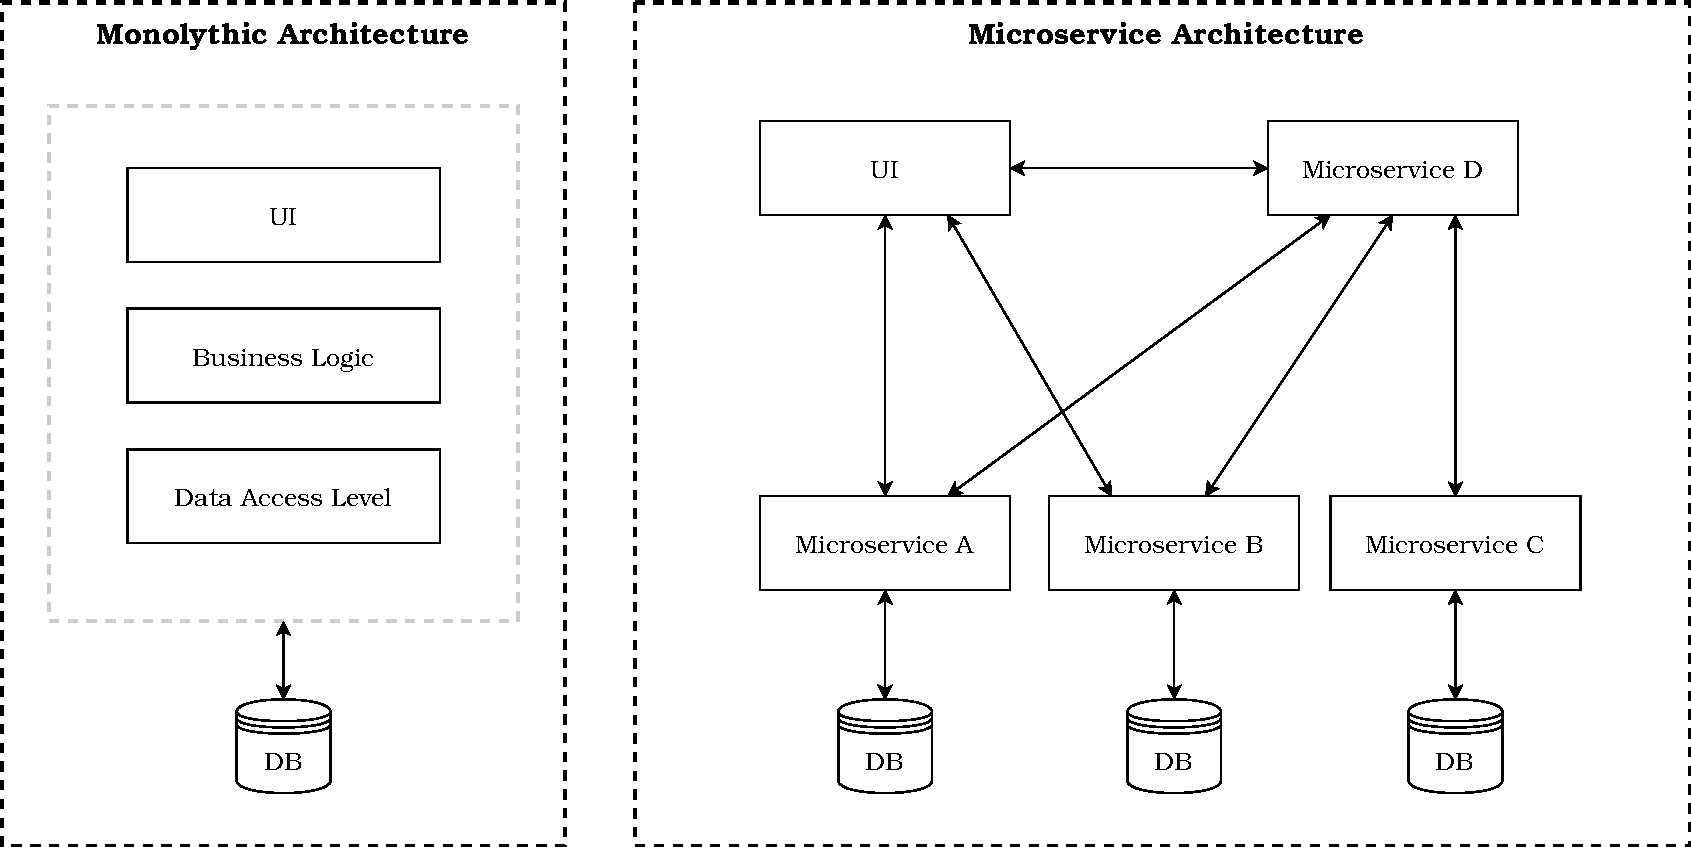
\includegraphics[width=\textwidth]{microservice-vs-monolyth.pdf}
  \caption{Monolythic vs. Microservice Architecture}
  \label{fig:microservice-vs-monolyth}
\end{figure*}

\subsection{Decentralized BaaS model}

According to McKinsey \& Co., there are three main trends in banking evolution:
\begin{itemize}
\item automation;
\item increased regulation;
\item increased pace of technological development.
\end{itemize}

Blockchain allows to automate different processes and banks can benefit from it a lot. Accounting, legal and risk parts might be automated. McKinsey \& Co. states that blockchain based on advanced cryptography might allow doing such operations the most effective, safe and transparent way in human history.

\paragraph*{For global players adaptation to such trends will become a vital issue.} More and more strict regulation of financial system will move players to use partner BaaS platforms as to adaptation to new jurisdictions independently will become too expensive. Fast tech development,  which most of the banks can’t handle, will drive banks interest in using other fintech companies services. It will drive a demand for BaaS usage.

\paragraph*{Decentralized BaaS is the future of banking. Why?} The world has changed and financial streams are becoming global. They are no longer easily controlled by common tools. Regulators, central banks defining the movement of the market are responding to this with more strict regulations. Banks respond by trying to take as many services as permitted by their license beyond their confines. They aim to create innovative services, leaving only themselves with just the core.

This trend creates the risk of a bank evolving into something more similar to a telecommunication company~--- a company with a license that no longer sees its clients.

At BankEx we see this risk, but believe it is right for banks to preserve the status of the most important key element of the world’s financial ecosystem. Fintech and IT companies should not be disrupters of the banking system. Instead they should supplement each other in a mutually beneficial way.

Several years ago banks and innovative technologies existed separately, with banks expressing an interest in external IT products such as certain separate features. Today the market has changed, leading banks of the world work more and more closely with fintech companies, while the fintech companies in turn ceased to see themselves as disruptors triumphing over banks and instead view themselves as partners to banks. Everyone acknowledges that offline bank departments will remain, even if nobody goes to them, as foundations of faith in the system. A customer must understand that the financial service he receives is that of a bank, the bank actually exists, it has a department in the city, to which the customer can go in case of an issue for assistance. This reason at least will remain. This isn’t just a domain that might close tomorrow and leave its end client alone with their issue. On the other hand, fintech and blockchain companies acknowledge that the market share occupied by their products is too small, below 10\%, and in order to amplify it they must partner with banks.

In other words, fintech products must end up at banks. Clients, in turn, will purchase and use innovational financial products much more willingly if they can do so under the brand of a familiar bank. It’s worth noting that there exist banks that are skeptical about integration with fintech companies. Luckily there are many banks and many of them understand that refusing innovations leads to them losing both clients and market share.

On the other hand, existing technologies are not enough for a tight collaboration on a market where the main product are large volumes of money and vast financial streams. Banks don’t trust one another and they don’t trust technological companies. They are afraid of losing their client-base by partnering with a stronger or more technologically advanced player. They are afraid that upon close examination their products will not be competitive compared to alternatives. They are afraid regulators would penalize them for use of innovations in their base products. Another important note is that decisions regarding such risks are made by top-managers, who need to keep their personal reputation in mind.

Technological progress has presented us with solutions to such issues~--- organizing mutual trust of participants in the system and trust in operations in the system based on decentralized data storage and automated smart-contracts.

Many professional market players admit that a decentralized BaaS business-model is an optimal path to collaboration between classic banks and financial companies with cutting edge IT companies and continually growing decentralized technological companies of the future.

Front service of clients remains in the hands of the banks, while products are presented by narrowly-oriented product banks or companies.

We believe that the \textit{B2B2C} combination of business-models and technologies is the key to BankEx’s success.

\subsection{Blockchain Serviсe Architecture (\textit{BlockchainService})}

On an Ethereum blockchain micro-service architecture is used in the implementation of external oracles. At the same time, the Ethereum network is itself an example of network that uses the concept of micro-services, since it contains all the characteristic features of micro-services:
\begin{itemize}
\item excess and reservation, as each node of the network is autonomous;
\item service discovery for automatic configuration of network topology;
\item extensibility through the use of other types of micro-services (such as oracles, micro-services allowing to display statistics, etc.). 
\end{itemize}

\begin{figure*}
  \centering
  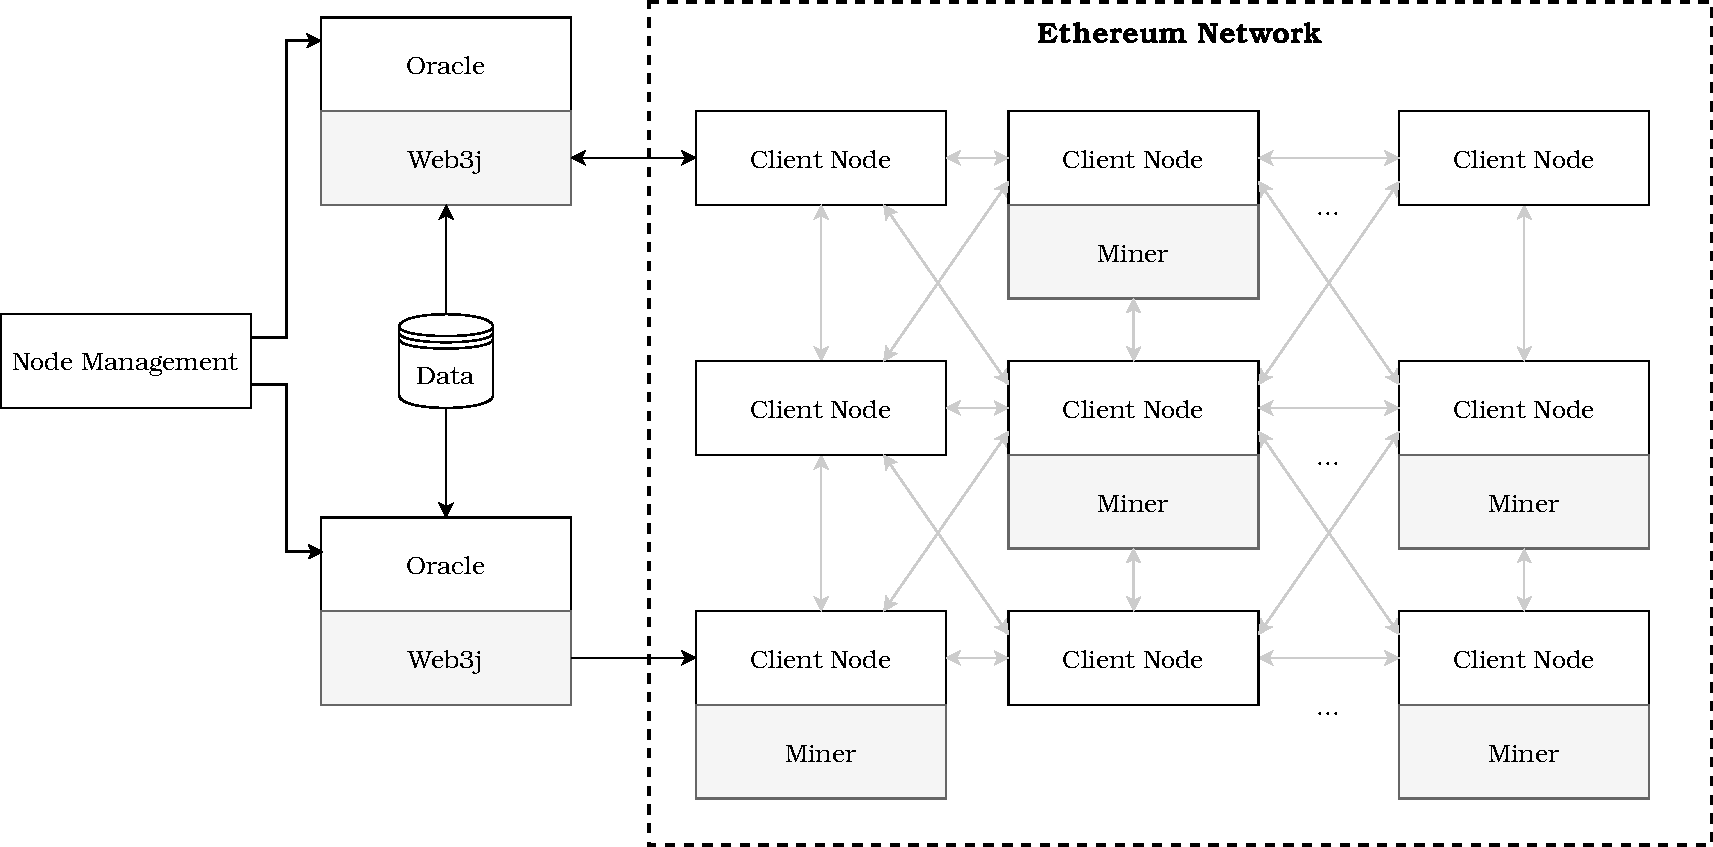
\includegraphics[width=\textwidth]{blockchain-microservice-architecture.pdf}
  \caption{Blockchain Service Architecture}
  \label{fig:blockchain-microservice-architecture}
\end{figure*}

The logic of the BankEx liquidity protocol is based on the concept of the Ethereum smart contract, and accordingly uses all of its infrastructure advantages. At the same time, technically, the BankEx protocol is a series of smart contract updates, however these smart contract updates are not micro-services themselves, the micro-services are in relation between API calls themselves. From our side, the business tasks of the protocol, which require a classical micro-service architecture, are realized through the creation of the oracle system. Protocol oracles are designed strictly according to the principles of the micro-services, that is, the instances of these oracles should be automatically added under the required conditions. In this case, dynamic balancing of the number of oracle instances is used. Part of the BankEx oracles is implemented on the basis of Microsoft Azure cloud technologies, since it’s one of the most bank friendly platforms. An example of the protocol logic was realized through the interaction with the signals from Internet of Things sensors.

But for the description of the BankEx Proof-of-Asset protocol the definition of the micro-service architecture is not entirely correct. BankEx team calls it the Blockchain Service Architecture. 

\paragraph*{Blockchain Service Architecture} is a sequence of smart contracts, every step of which can be customized by a predetermined pool of actors validated for the particular step of the included smart contracts, while the contents of contracts in a step and the number of steps are embedded in the business logic necessary to tokenize the Smart Asset. 

\paragraph*{Blockchain Serviсe Architecture} is an asset tokenization constructor, but one that only works in a sequence of smart contracts correctly arranged after one another, supplemented with oracles connected as micro-services. 

This allows to tokenize an asset with maximum precision and transparency for all participants of the market, while also working in line with the open source BankEx Proof-Of-Asset protocol.

\subsection{Complexity regulation of the Blockchain Serviсe Architecture (\textit{BlockchainServiсe})}

We often hear from technical experts: Your protocol is too complicated. Other technical gurus say~--- your protocol is too simple. Yes, they are correct. The complexity of the BankEx protocol, which is based on the Blockchain Service Architecture, is regulated by the increase/decrease in the number of smart contracts in the tokenization logic. 

The creation of a smart asset of a certain type does not necessary use all the steps that are laid out in the BlockSA, only the steps of the smart contract chain that are required by a particular Smart Asset are used. The simplest Smart Asset consists of three steps: initialization, validation, and valuation. And in this case the Smart Asset will fulfill its mission - make the asset liquid. It’s not complicated at all. 

At the same time, BankEx is an old company in the sphere of financial technologies, classic fintech. We know very well how complex financial tools can be, and how difficult it is to properly formalize them. Our solution is the Blockchain Service Architecture – exactly what you need. You can add any level of complexity to the asset tokenization chain which will result in a Smart Asset.

Moreover, the Smart Asset retains all the features of a blockchain Smart Contract - everyone is able to see what value is behind it and how truthful it is. 

You can add your own logic block to the BlockchainService chain - Proof-of-Asset Protocol, because it is an open source code. To do that – you will need to address the BankEx Foundation community.


\subsection{What is Blockchain Serviсe Architecture (BlockSA)}

\subsection{Liquidity Theory Through the Prizm of Tokenization}

\subsection{Market Making Mathematical Models for Smart Asset}



\end{multicols}

\newpage
\appendix

\section{Terminology}
\begin{description}
\item[Blockchain]~--- is a continuously growing list of records, called \textit{blocks}, which are linked and secured using cryptography \cite{bitcoinComprehensive2016} \cite{wikipediaBlockchain}.
\item[Tokenization]~--- process of converting rights into digital token to be circulated onver blockchain with low transactional fees. Tokenization is a blockchain equivalent of securitization.
\end{description}

\printbibliography

\end{document}
